\textbf{Цель работы:} предполагается изучить спектр гамма-излучений для образцов $\mathrm{^{22}Na, \; ^{137}Cs, \; ^{60}Co, \; ^{241}Am}$ и $\mathrm{^{152}Eu}$, найти для них пики полного поглощения и обратного рассеяния.

\textbf{Используемое оборудование}: сцинтиллятор, ФЭУ, предусилитель импульсов, высоковольтный блок питания для ФЭУ, АЦП, компьютер.
             
\section{Теоретическое введение}

    \textbf{Фотоэффект} -- это процесс взаимодействия гамма-кванта с электроном, связанным с атомом, при котором электрону передается вся энергия гамма-кванта. При этом электрону сообщается кинетическая энергия $T_e = E_\gamma - E_i$, где $E_\gamma$ -- энергия гамма-кванта, $E_i$ -- потенциал ионизации $i$-той оболочки атома. Фотоэффект особенно существенен для тяжелых веществ, где он идет с заметной вероятностью даже при высоких энергиях гамма-квантов. В легких веществах фотоэффект становится заметен лишь при относительно небольших энергиях гамма-квантов.

    \textbf{Эффект Комптона} - это упругое рассеяние фотона на свободном электроне, сопровождающееся изменением длины волны фотона. Максимальная энергия образующихся комптоновских электронов соответствует рассеянию гамма-квантов на $180^\circ$ и равна
    \begin{equation}
        E_{\max}=\frac{\hbar\omega}{1+\frac{mc^2}{2\hbar\omega}}.
    \end{equation}

    \textbf{Процесс образования электрон-позитронных пар.}
    При достаточно высокой энергии гамма-кванта наряду с фотоэффектом и эффектом Комптона может происходить третий вид взаимодействия гамма-квантов с веществом -- образование электрон-позитронных пар. Процесс образования пар не может происходить в пустоте, так как в этом случае не выполняются законы сохранения энергии и импульса. В присутствии ядра или электрона процесс образования пары гамма-квантов возможен, так как можно распределить энергию и импульс гамма-кванта между тремя частицами без противоречия с законами сохранения. При этом если процесс образования пары идет в кулоновском поле ядра или протона, то энергия образующегося ядра отдачи оказывается весьма малой, так что пороговая энергия гамма-кванта $E_0$, необходимая для образования пары, практически совпадает с удвоенной энергией покоя электрона $E_0\cong 2mc^2=1.022$ МэВ.\par
    Появившийся в результате процесса образования пар электрон свою энергию на ионизацию среды. Таким образом, вся энергия электрона остается в детекторе. Позитрон будет двигаться до тех пор, пока практически не остановится, а затем аннигилирует с электроном среды, в результате чего появятся два гамма-кванта. То есть, кинетическая энергия позитрона также останется в детекторе. Далее возможны три варианта развития событий:

    \begin{enumerate}
        \item Оба родившихся гамма-кванта не вылетают из детектора, и тогда вся энергия первичного гамма-кванта останется в детекторе, а в спектре появится пик с $E=E_{\gamma}$;
        \item Один из родившихся гамма-квантов покидает детектор, и в спектре появляется пик, соответствующий энергии $E=E_{\gamma} - E_0$, где $E_0 = mc^2=511$ кэВ;
        \item Оба родившихся гамма-кванта покидают детектор, и в спектре появляется пик, соотвествующий энергии $E = E_{\gamma} - 2E_0$, где $2E_0 = 2mc^2= 1022$ кэВ.
    \end{enumerate}

    Таким образом, любой спектр, получаемый с помощью гамма-спектрометра, описывается несколькими компонентами, каждая из которых связана с определенным физическим процессом. Как описано выше, основными физическими процессами взаимодействия гамма-квантов с веществом является фотоэффект, эффект Комптона и образование электрон-позитронных пар, и каждый из них вносит свой вклад в образование спектра. Помимо этих процессов, добавляется \textit{экспонента}, связанная с наличием фона, \textit{пик характеристического излучения}, возникающий при взаимодействии гамма-квантов с окружающим веществом, а также \textit{пик обратного рассеяния}, образующийся при энергии квантов $E_{\gamma}\gg mc^2/2$ в результате рассеяния гамма-квантов на большие углы на материалах  конструктивных элементов детектора и защиты. Положение пика обратного рассеяния определяется по формуле:

    \begin{equation}
        E_{\text{обр}} = \frac{E}{1 + \frac{2E}{mc^2}},
        \label{eq:Ereverse}
    \end{equation}
    где $E$ -- энергия фотопика.

    \textbf{Энергетическое разрешение спектрометра.} Даже при поглощении частиц с одинаковой энергией амплитуда импульса на выходе фотоприёмника сцинтилляционного детектора меняется от события к событию. Это связано:
    \begin{enumerate}
        \item Со статистическим характером процессов сбора фотонов на фотоприёмнике и последующего усиления,
        \item С различной вероятностью доставки фотона к фотоприемнику из разных точек сцинтиллятора,
        \item С разбросом высвечиваемого числа фотонов
    \end{enumerate}

    В результате в набранном спектре линия (которая для идеального детектора представляла бы дельта-функцию) оказывается размытой, её часто описывают гауссианом.
    
    Энергетическим разрешением спектрометра называется величина
    \begin{equation}
        R_i=\frac{\Delta E_i}{E_i},
    \end{equation}
    где $\Delta E_i$ -- ширина пика полного поглощения, измеренная на половине высоты, $E_i$ -- энергия регистрируемого $\gamma$-излучения. Значение $E_i$ пропорционально среднему числу фотонов $\overline{n_i}$ на выходе ФЭУ, т.е.:
    \begin{equation}
        E_i = \alpha\overline{n_i}.
        \label{eq:4}
    \end{equation}

    Полуширина пика полного поглощения $\Delta E_i$ пропорциональна среднеквадратичной флуктуации $\overline{\Delta n_i}$. Т.к. $n_i$ является дискретной случайной величиной, которая распределена по закону Пуассона, то $\overline{\Delta n_i}=\sqrt{\overline{n_i}}$ и поэтому
    \begin{equation}
        \Delta E_i = \alpha\overline{\Delta n_i} = \alpha\sqrt{\overline{n_i}}.
        \label{eq:5}
    \end{equation}

    Из (\ref{eq:4}), (\ref{eq:5}) получаем, что
    \begin{equation}
        R_i = \frac{\Delta E_i}{E_i} = \frac{\text{const}}{\sqrt{E_i}}.
        \label{eq:6}
    \end{equation}

    Поскольку энергетическое разрешение зависит от энергии, его следует указывать для конкретной энергии. Чаще всего разрешение указывают для энергии гамма-линии $^{137}\text{Cs}$ (661.7 кэВ).

\section{Ход работы}
\subsection{Измерение значений фотопиков}

    Снимем энергетические спектры с помощью экспериментальной установки для образцов $\mathrm{^{22}Na, \; ^{137}Cs, \; ^{60}Co, \; ^{241}Am}$ и $\mathrm{^{152}Eu}$.

    \begin{figure}[H]
        \centering
        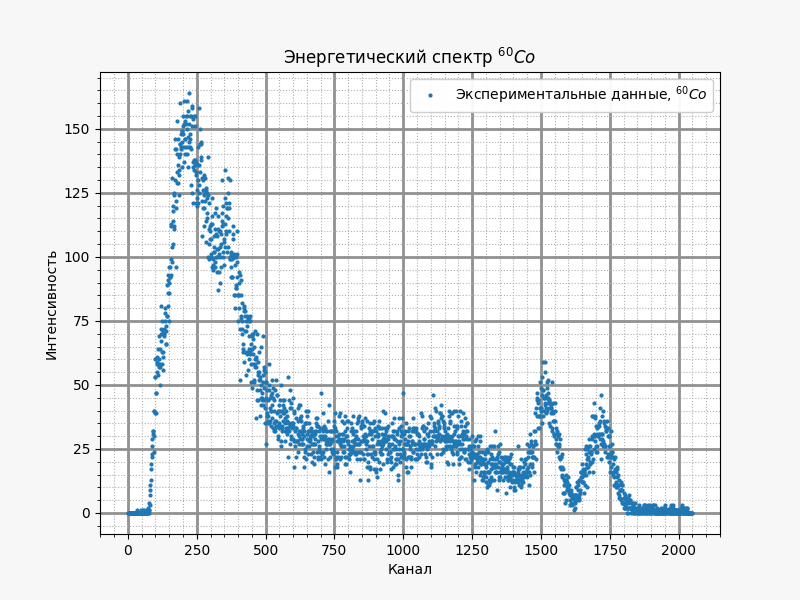
\includegraphics[width = 12 cm]{images/Co60}
        \caption{Энергетический спектр, измеренный для образца $^{60}Co$}
        \label{Co60_pic}
    \end{figure}

    \begin{figure}[H]
        \centering
        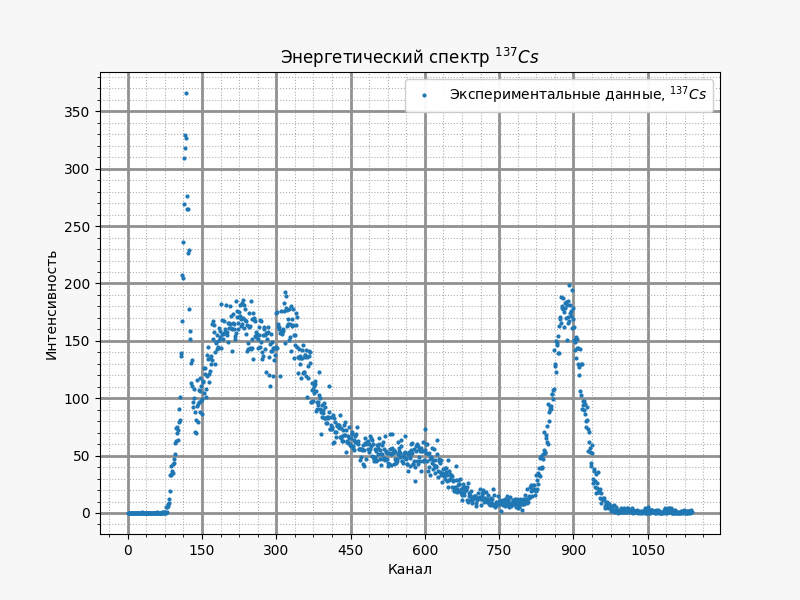
\includegraphics[width = 12 cm]{images/Cs137}
        \caption{Энергетический спектр, измеренный для образца $^{137}Cs$}
        \label{Cs137_pic}
    \end{figure}

    \begin{figure}[H]
        \centering
        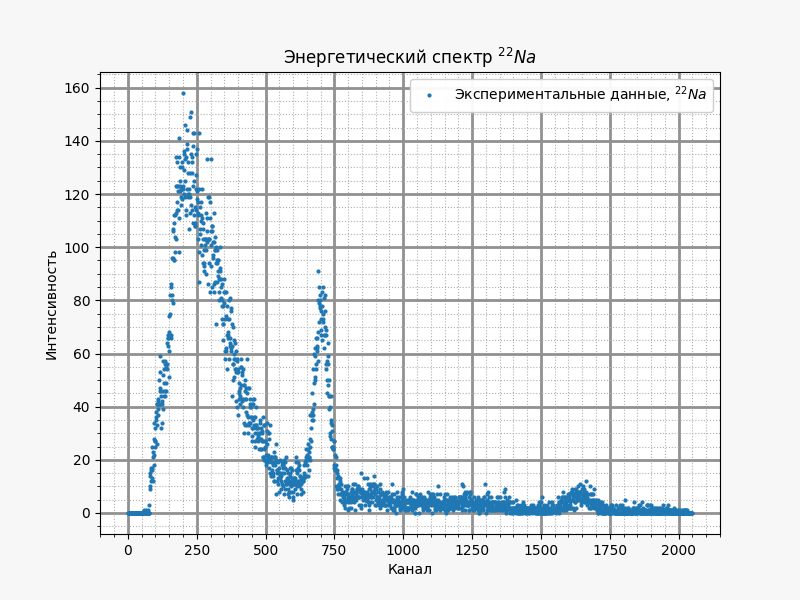
\includegraphics[width = 12 cm]{images/Na22}
        \caption{Энергетический спектр, измеренный для образца $^{22}Na$}
        \label{Na22_pic}
    \end{figure}

    \begin{figure}[H]
        \centering
        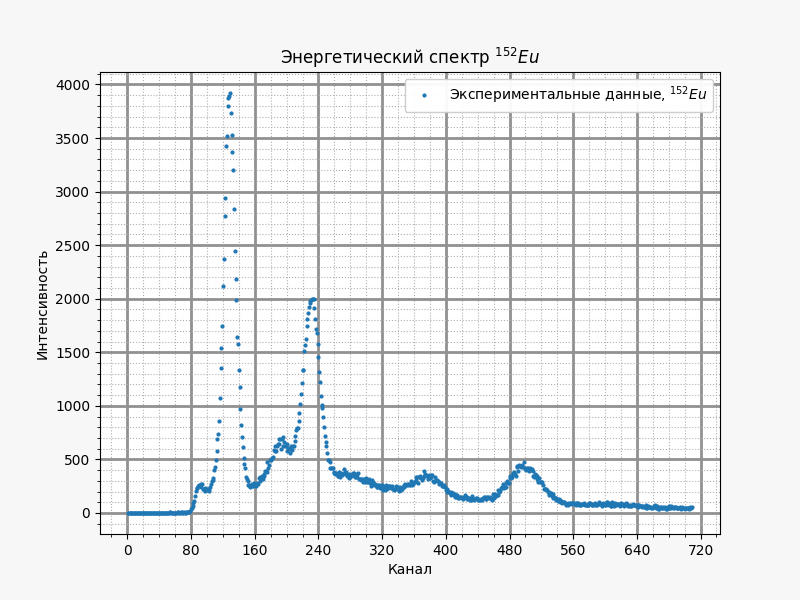
\includegraphics[width = 12 cm]{images/Eu152}
        \caption{Энергетический спектр, измеренный для образца $^{152}Eu$}
        \label{Eu152_pic}
    \end{figure}

    \begin{figure}[H]
        \centering
        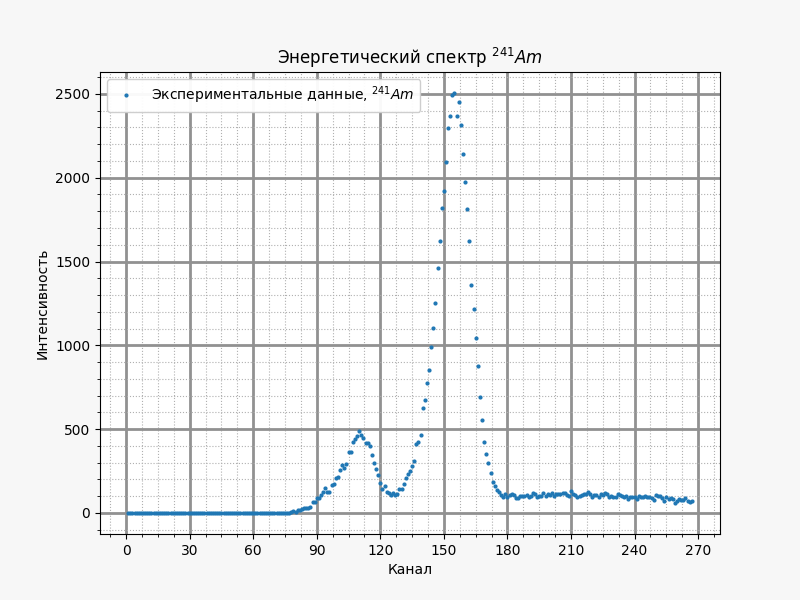
\includegraphics[width = 12 cm]{images/Am241}
        \caption{Энергетический спектр, измеренный для образца $^{241}Am$}
        \label{Am241_pic}
    \end{figure}

    \begin{figure}[H]
        \centering
        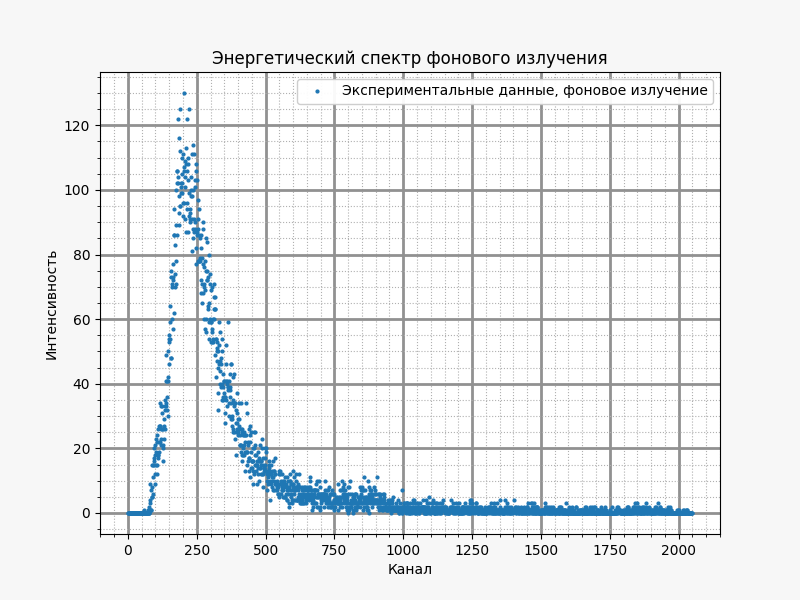
\includegraphics[width = 12 cm]{images/background}
        \caption{Энергетический спектр фонового излучения}
        \label{back_pic}
    \end{figure}

    По значениям каналов у пиков полного поглощения излучения от радиоактивных источников $^{60}Co, \; ^{137}Cs, \; ^{22}Na$ определим калибровочную формулу перехода со значений каналов к значениям энергий:

    \begin{table}[H]
        \centering
        \begin{tabular}{|c|c|c|c|c|c|}
        \hline
        Элемент  & $^{60}Co$ & $^{60}Co$ & $^{137}Cs$ & $^{22}Na$ & $^{22}Na$ \\ \hline
        $N_i$      & 1524      & 1716      & 887       & 706       & 1653    \\ \hline
        $E_i$, МэВ & 1.173     & 1.332     & 0.662     & 0.511     & 1.274   \\ \hline
        \end{tabular}
    \end{table}

    \begin{equation}
        E = aN + b, \; a = 711 \; \text{эВ}, b = 27.609 \; \text{КэВ}
    \end{equation}

    По полученной формуле посчитаем значения для пиков поглощения для различных материалов, а также ширину самих пиков.

    \begin{table}[h!]
        \centering
        \caption{Пики полного поглощения различных образцов}
        \label{tab:peaks}
        \begin{tabular}{|c|c|c|c|c|c|}
            \hline
            Элемент & $N_i$ & $\triangle N_i$ & $E_i$, МэВ & $\triangle E_i$, МэВ & $R_i$  \\
            \hline
            $^{22}$Na & 706 & 46 & 0.530 & 0.033 & 0.063 \\
            \hline
            $^{22}$Na & 1653 & 83 & 1.204 & 0.059 & 0.049  \\
            \hline
            $^{60}$Co & 1524 & 82 & 1.112 & 0.058 & 0.052  \\
            \hline
            $^{60}$Co & 1716 & 86 & 1.248 & 0.061 & 0.049 \\
            \hline
            $^{137}$Cs & 887 & 55 & 0.659 & 0.039 & 0.059  \\
            \hline
            $^{241}$Am & 155 & 16 & 0.138 & 0.011 & 0.079  \\
            \hline
            $^{152}$Eu & 232 & 21 & 0.192 & 0.015 & 0.078 \\
            \hline
            $^{152}$Eu & 376 & 29 & 0.295 & 0.021 & 0.071  \\
            \hline
            $^{152}$Eu & 498 & 37 & 0.382 & 0.026 & 0.068 \\
            \hline
        \end{tabular}
    \end{table}

\subsection{Проверка формулы энергетического разрешения}
    
    Построим график зависимости $R_i^2(1/E_i)$. Из линейно аппроксимации графика получим значения для коэффициента корелляции $R^2 = 0.949$, что означает справедливость линейной аппроксимации, а значит исходную зависимость можно считать линейной.

    \begin{figure}[H]
        \centering
        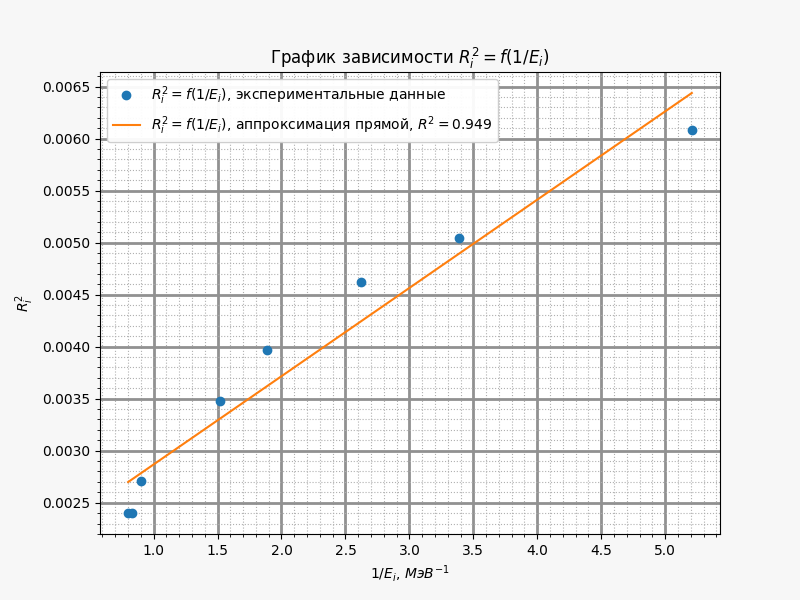
\includegraphics[width = 14 cm]{images/R2_and_invE}
        \caption{График зависимости $R_i^2(1/E_i)$}
        \label{R2_and_invE}
    \end{figure}

\subsection{Проверка формулы для края комптоновского спектра}

    Измерим из энергетических кривых значения комптоновских краев. 

    \begin{table}[h!]
        \centering
        \begin{tabular}{|c|c|c|c|c|c|}
            \hline
            Элемент                         & $^{60}Na$ & $^{60}Co$ & $^{60}Cs$ & $^{152}Eu$ & $^{152}Eu$ \\ \hline
            $E_i,$ МэВ                      & 1.204     & 1.112     & 0.662     & 0.192      & 0.295      \\ \hline
            $E_{\text{комп}}$               & 0.966     & 0.874     & 0.460     & 0.087      & 0.165      \\ \hline
            $E_{\text{комп}}^{\text{теор}}$ & 0.993     & 0.904     & 0.475     & 0.082      & 0.158      \\ \hline
        \end{tabular}
    \end{table}

    \begin{figure}[H]
        \centering
        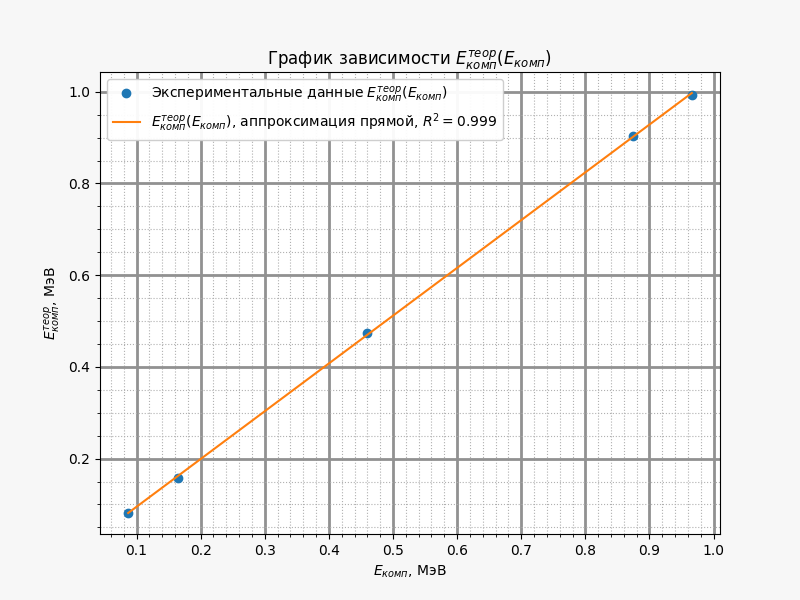
\includegraphics[width = 13 cm]{images/E_compton}
        \caption{График зависимости $E_{\text{комп}}^{\text{теор}}(E_{\text{комп}})$}
        \label{E_compton}
    \end{figure}

    Таким образом, имеем коэффициент корелляции для зависимости $R^2 = 0.999$, причём коэффициент линейной зависимости равен $k = 1.042 \pm 0.012$, значит можно считать теоретическую формулу для эффекта Комптона верной. При сравнении значений использовались не все доступные значения, так как ввиду большого статистического разброса для некоторых комптоновских краев невозможно определить значение энергии, им соответствующее.
    
\subsection{Проверка формулы для пиков энергии обратного рассеяния}

    Для энергетических спектров, для которых возможно измерить значения обратного фотопика, построим график зависимости $E_{\text{обр}}^{\text{теор}}(E_{\text{обр}})$.

    \begin{table}[H]
        \centering
        \begin{tabular}{|c|c|c|c|}
            \hline
            Элемент                        & $^{60}Co$ & $^{60}Cs$ & $^{152}Eu$ \\ \hline
            $E_i,$ МэВ                     & 1.112     & 0.662       & 0.295      \\ \hline
            $E_{\text{обр}}$               & 0.203     & 0.184       & 0.163      \\ \hline
            $E_{\text{обр}}^{\text{теор}}$ & 0.212     & 0.190       & 0.153      \\ \hline
        \end{tabular}
    \end{table}

    \begin{figure}[H]
        \centering
        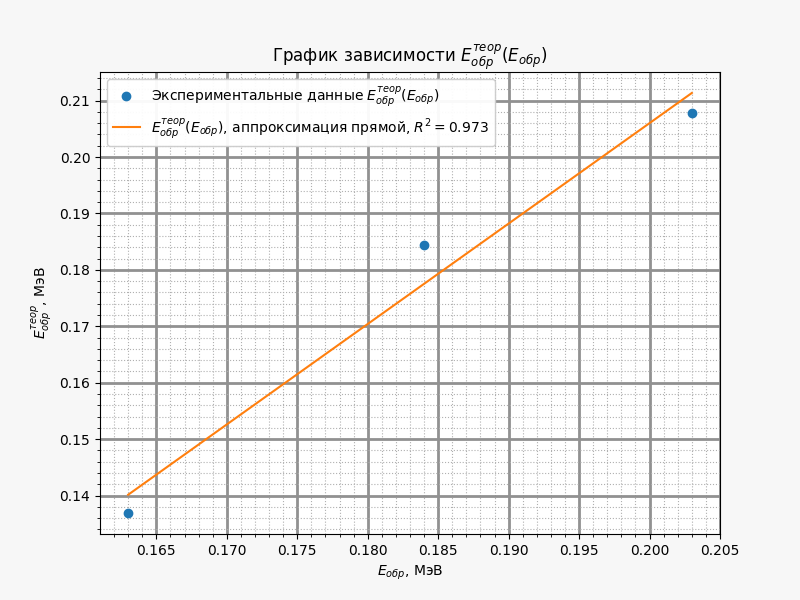
\includegraphics[width = 13 cm]{images/E_inv}
        \caption{График зависимости  $E_{\text{обр}}^{\text{теор}}(E_{\text{обр}})$}
        \label{E_inv}
    \end{figure}

    Таким образом, из графика видно, что зависимость можно считать линейной, так как коэффициент кореллляции равен $R^2 = 0.973$. При этом линейный коэффициент равен $k = 0.948 \pm 0.243$.

\subsection{Характеристическое излучение свинца}    

    По графикам определим энергию характеристического излучения свинца, служащего защитой спектрометра от внешнего излучения. На всех спектрах, в той или иной степени выражена спектральная линия, соответствующая энергии 84 КэВ. Эта энергия и есть энергия характеристического излучения свинца. Особенно хороша она видна на графике европия.

\subsection{Импульсы на выходе ФЭУ}

    Осцилограмма импульсов на выходе ФЭУ имеет вид
    \begin{equation}
        U(t) = const \cdot e^{-\frac{t}{RC}} \left( 1 - e^{-\frac{t}{\tau_0}} \right),
    \end{equation}
    где $\tau_0$ -- время высвечивания сцинтиллятора, а $RC$ -- постоянная времени, $RC \gg \tau_0$.

    Осциллограф показывает графики следующих видов:
    \begin{figure}[H]
        \centering
        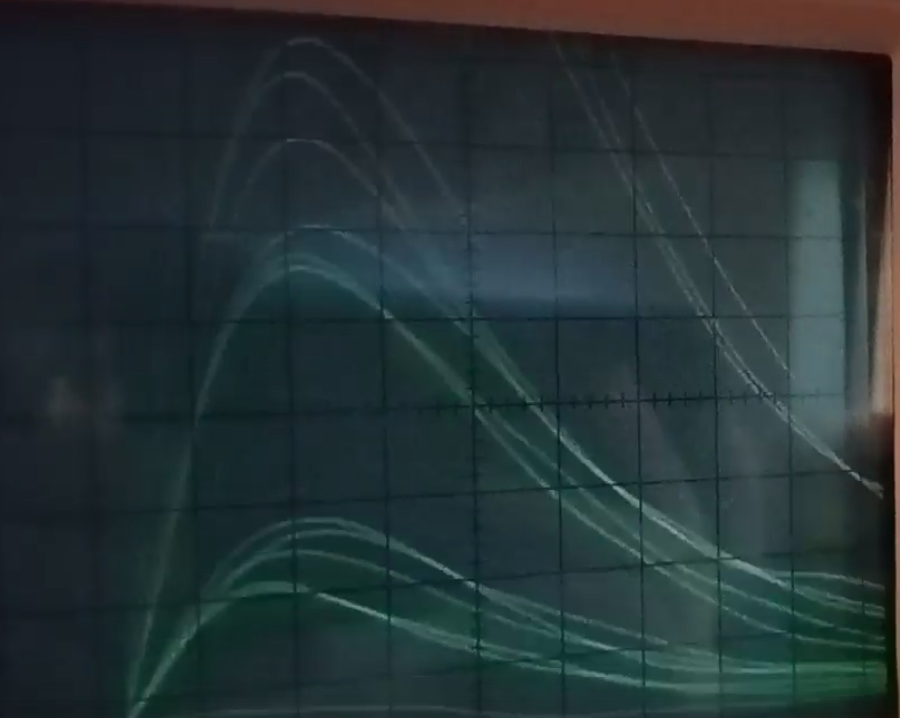
\includegraphics[width = 13 cm]{images/RC}
        \caption{Графики импульсов на выходе ФЭУ}
        \label{RC}
    \end{figure}

    По преденему фронту импульса можно оценить $\tau_0$:
    \begin{equation}
        U(t) \approx const \left( 1 - e^{-\frac{t}{\tau_0}} \right) \approx const \cdot \frac{t}{\tau_0}.
    \end{equation}

    Таким образом, $\tau_0$ можно оценить по прекращению нарастания импульса (т.е. на моменте, когда вырождается линейная зависимость): $\tau_0 = 1.8$ мкс. 

    По заднему фронту оценим $RC$, зафиксировав момент спада сигнала в $e$ раз: $RC = 5.2$ мкс.
    
\section{Заключение}

    Таким образом, в работе измерены спектры гамма-излучений для образцов $\mathrm{^{22}Na, \; ^{137}Cs, \; ^{60}Co, \; ^{241}Am}$ и $\mathrm{^{152}Eu}$, найдены для них пики полного поглощения, обратного рассеяния, а также комптоновские края. Проверены формулы для пиков обратного рассеяния и комптоновских краев.

    Найдено значение характеристического излучения свинца, служащего защитой спектрометра от внешнего излучения, равное 84 КэВ.

    По форме импульсов на выходе ФЭУ оценены время высвечивания сцинтиллятора $\tau_0 = 1.8$ мкс, а также $RC = 5.2$ мкс -- постоянная времени цепи на выходе ФЭУ.
